
\section{Mutual Information Estimation}

As stated before we are trying to validate the fact that compression is
happening within the hidden layers in a neural network as such having robust
tools to measure mutual information is of utmost importance. 

\subsection{Mutual Information Definition}

Mutual information is a measure of dependence between two variables $ X $ and $
Y $, it quantifies the number of bits obtained about one when observing the
other.

Suppose we have two random variables $ X $ and $ Y $ if we want to measure
mutual information between the two of them we usually refer to one of the
following equations:

\medskip

Using the entropy of the distributions to infer the value
\begin{equation}
  I(X, Y) = H(X) - H(X|Y)
\end{equation}
\begin{equation}
  I(X, Y) = H(X) + H(Y) - H(X,Y)
\end{equation}

Or calculating the mutual information explicitly from probabilities, for
discrete and continuous distributions respectively
\begin{equation}
      {I} (X;Y)=\sum _{y\in {\mathcal {Y}}}\sum _{x\in {\mathcal
      {X}}}{p(x,y)\log {\left({\frac {p(x,y)}{p(x)\,p(y)}}\right)}} 
\end{equation}

\begin{equation}
    {I} (X;Y)=\int _{\mathcal {Y}}\int _{\mathcal {X}}{p(x,y)\log {\left({\frac
    {p(x,y)}{p(x)\,p(y)}}\right)}}\;dx\,dy
\end{equation}


\subsection{Theoretically undefined}

Calculating mutual information is mathematically defined for both continuous and
discrete distributions by using one of the functions above. However since we are
looking at neural networks we do not have the full distribution -- only an
empirical sample of the unknown joint distribution $ P(X,Y) $. As such we cannot
use conventional methods to calculate the mutual information and instead have to
use tools to estimate it.

The field of estimating mutual information is relatively new as a result the
tools that are available are quite primitive. There has been some papers
published that use more advanced techniques to tackle the problem, we will talk
about in \autoref{ssection:advanced}

\section{Calculating Mutual Information}

\subsection{Experimental setup}

\begin{figure}[H]
    \begin{pythonfigure}
      Algorithm: Generate Information Plane Data
      Input:
      ;$T$; = number of layers
      ;$X$; = training data
      ;$Y$; = label data
      N = number of epochs
      Output: 
      ;$I_x$;(epoch, layer), # mutual information with $X$ 
      ;$I_y$;(epoch, layer)  # mutual information with $Y$ 
      Algorithm:
      NN = setup_neural_network(;$T$;, ;$X$;, ;$Y$;)
      for e in 0..N:
        NN.run_SGD_once()
        for t in 0..;$T$;:
          data = []
          for ;$x \in X$;:
            ;$\hat{t}$; = NN.predict(;$x$;).layer_activation(t)
            data.append(;$\hat{t}$;)
          ;$I_x$;(e, t) = calculate_mutual_information(data, ;$X$;)
          ;$I_y$;(e, t) = calculate_mutual_information(data, ;$Y$;)
    \end{pythonfigure}
    \caption{The general algorithm for calculating mutual information inside a
    neural network.}
    \label{fig:general}
\end{figure}

\begin{itemize}
  \item{
      X input is an empirical sample of all possible inputs.
    }
  \item{
      Y label data. Every $x \in X$ has a corresponding label $y \in Y$. 
    }
  \item{
      $T_{e,i}$ data for a specific epoch $e$ and specific layer $i$ in the
      neural network. The dataset is  generated by feeding every $x \in X$
      trough the neural network and recording the activations.
    }
\end{itemize}

\newpage

\subsection{Discrete method} 

  The method used by Tishby in his paper. The method estimates mutual
  information between the $X$ or $Y$ and the hidden layer $T$ by assuming the
  observed empirical distribution of input samples is the true distribution. We
  use this assumption to compute entropies of $T$ and varying subsets as
  outlined in \autoref{eq:discrete}

\begin{equation}
  I(X, Y) = H(X) - H(X|Y) = H(X) - \sum _{y\in Y} H(X|Y = y)p(Y = y)
\label{eq:discrete}
\end{equation} 


  However just calculating mutual information for a discrete distribution is not
  enough as this yields mutual information equal to 0, in order to sidestep this
  issue we need to simulate randomness Tishby achieves this by grouping multiple
  values together, which he calls binning. A more detailed explanation why this
  is done is given in \autoref{ssection:detnet}

   \autoref{fig:mutualinfo} trough to \autoref{fig:entropy2} outline the full
   algorithm.
\begin{figure}[H]
    \begin{pythonfigure}
      Algorithm: Mutual Information
      Input: 
      ;$X = x_1, x_2,...,x_n$;
      ;$Y = y_1, y_2,...,y_n$;
      Output: ;$I(X:Y)$;
      ;$X$; = Bin close values of ;$X$; together
      ;$Y$; = Bin close values of ;$Y$; together
      ;$H(X)$; = Calculate entropy of X
      ;$H(X|Y)$; = Calculate conditional entropy of X given Y
      ;$I = H(X) - H(X|Y)$;
    \end{pythonfigure}
    \caption{Pseudo code for computing mutual information refer to
    \autoref{fig:entropy1} and \autoref{fig:entropy2} for entropy computation.}
    \label{fig:mutualinfo}
\end{figure}

\begin{figure}[H]
    \begin{pythonfigure}
      Algorithm: Entropy - Discrete Method
      Input: ;$X = x_1, x_2,...,x_n$;
      Output: ;$H(X)$;
      for ;$ \hat{x}\in Unique(X)$;:
        count = 0       
        for ;$x \in X$;:
          if ;$\hat{x} = x$;:
            count = count + 1
        ;$P_x$; = count / len;$(X)$;
      ;$H(X) = - \sum _{x\in Unique(X)} P_x log(P_x)$; 
    \end{pythonfigure}
    \caption{Algorithm for computing entropy -- Discrete method}
    \label{fig:entropy1}
\end{figure} 

\begin{figure}[H]
    \begin{pythonfigure}
      Algorithm: Conditional Entropy
      Input: 
      ;$X = x_1, x_2,...,x_n$;
      ;$Y = y_1, y_2,...,y_n$;
      Output: ;$H(X|Y)$;
      ;$H(X|Y) = H(X)$;
      for ;$ \hat{y}\in Unique(Y)$;:
        ;$\hat{X}$; = []
        for ;$x, y \in zip(X, Y)$;:
          if ;$\hat{y} = y$;:
            ;$\hat{X}$;.append(;$x$;)
          ;$H(X|Y) = H(X|Y) - H(\hat{X})$;
    \end{pythonfigure}
    \caption{Algorithm for computing conditional entropy}
    \label{fig:entropy2}
\end{figure}

When computing mutual information between a hidden layer $T$ and the input set
$X$ we can abuse the fact that every element $x\in X$ is unique and uniquely
identifies an element $t\in T$ hence 

\begin{equation}
  H(T|X) = 0 
\end{equation}

\begin{equation}
  I(T, X) = H(T) - H(T|X) = H(T) 
\end{equation}

This does not affect the result but increases performance of our algorithm.

\subsection{Kernel Density Estimation}

  The KDE method used in Saxe's paper but originally devised by Kolchinsky \&
  Tracey (2017); Kolchinsky et al. (2017). As well as the Discrete method KDE
  assumes that the observed empirical distribution in the hidden layer $T$ is
  the true distribution. 

  However, instead of binning values together KDE assumes the distribution is a
  mixture of Gaussians. Using this fact we can get an upper bound when
  calculating entropy for a collection of data points.

  The algorithm closely follows figures :\autoref{fig:mutualinfo},
  \autoref{fig:entropy1}, and \autoref{fig:entropy2}, however there is a change
  the way entropy is calculated so instead of \autoref{fig:entropy1} we have
  \autoref{fig:entropy3} below.

\begin{figure}[H]
    \begin{pythonfigure}
      Algorithm: Entropy - KDE
      Input: 
      ;$X = x_1, x_2,...,x_n$;  
      var = noise variance 0.05 by default
      Output: ;$H(X)$;
      dists = compute distance matrix of ;$X$;
      dists = dists / 2*var # divide every distance by a value
      # an $x$ is an observation of a hidden layer so, hence it's a vector 
      # which has an associated dimension
      dim = ;$x_1$;.dimension
      normconst = (dim / 2)*log(2*;$\pi$;*var)
      lprobs = []
      for row in dists:
        lprobs.append(log(sum(exp(-row))) - log(n) - normconst
      H(X) = mean(lprobs) + (dim / 2)
    \end{pythonfigure}
    \caption{Algorithm for computing entropy -- Kernel Density Estimation method.
    The same algorithm as used by Saxe.}
    \label{fig:entropy3}
\end{figure} 

As before when computing mutual information between a hidden layer $T$ and the
input set $X$ we can use the fact that every element $x\in X$ is unique and
hence uniquely identifies an element in $t\in T$.

\subsection{Advanced methods} \label{ssection:advanced}

Since mutual information estimation is a contentious part of the project we
wanted to experiment with more advanced techniques however we were not able to
adopt the methods for this project, the methods that we have tried are outlined
below.

\subsubsection{Mutual Information by Gaussian approximation}
  
  "Estimating Mutual Information by Local Gaussian Approximation" (Shuyang Gao). A
  promising way to estimate mutual information. However the implementation
  proved to be to difficult and time consuming so we abandoned it. I contacted
  out to the author but he was not able to provide any concrete code.

\subsubsection{Geometrical Adaptive Entropy Estimation}

  "Breaking the Bandwidth Barrier: Geometric Adaptive Entropy Estimation"
  (Weihao Gao). We were pointed to this paper by S. Gao the author of the
  previous method, as previously this looked like a promising method to measure
  entropy and mutual information. Furthermore, the code was available online
  unfortunately we were not able to adapt the code for multidimensional values
  as a result we were getting wrong and inconsistent results. We decided making
  this method work would require too much time and is out of scope of this
  project.

\section{Implementation Optimizations}

Producing data for the information plane requires a substantial amount of
computational power and memory, in order for the computation to complete in a
reasonable amount of time we have to utilize all the available resources and
minimize the amount of work we are doing.

\subsection{Maximising Resource Utilization}

The obvious way to maximise the resource usage is to parllelize the workload.
If we refer to \autoref{fig:general}, we can see two main ways we can do this.

The first way is to parallelize one of the two outer loops and run mutual
information calculations in parallel, this is easy to do, however an issue
occurs if we need a lot of memory since every instance of mutual information
calculation manipulates the datasets creating copies, this is an issue for
bigger datasets such as MNIST.

The second way is to parallelize the mutual information calculation itself, this
is nice since we use minimal amounts of memory, however might be hard or
impossible to implement as it depends on the method.

The second way is to parallelize the mutual information calculation itself, this
method has a  bonus that uses minimal amounts of memory improving performance
for bigger datasets such as MNIST. However implementing this option might be
hard as it heavily depends on the maths of the method, or impossible if the
method has an inherently linear part to it. In our case KDE parallel performance
is very good, however Tishby's Discrete method has some bottlenecks that I
wasn't able to remove.

\subsection{Minimising the Workload}

Even when using all the systems resources the calculations take a very long
time to complete as such we need to find a way to speed it up. If we consider an
information plane graph for ex. \autoref{fig:ip1}, we see that from epoch to
epoch there is very little change that is occurring, skipping some epochs might
be a good way to reduce workload while keeping the overall result unchanged. We
have implemented a couple of ways to skip the epochs 

\subsubsection{Simple Skip}
  
  A very simple simple way to skip epochs calculates mutual information for
  every $n'th$ epoch.

  It's quite effective and is fast to implement and easy to parallelize, however
  it yields subpar results. At the beginning of the training period during the
  fitting phase the step sizes are too big and yields gaps in data as there are
  big changes between consecutive epochs. Toward the end of the training period
  during the compression phase the step size becomes too small and we are
  wasting computation as the changes between epochs is negligible. The next two
  methods address this problem, but have their own drawbacks.

\subsubsection{Delta Skip -- Exact}

  The Exact Delta Skip method introduces a distance metric which measures
  mutual information distance between two epochs. Using the distance metric the
  method tries to skip as many epochs as possible while still guaranteeing that
  the distance is at most delta $\delta$, and backtracks when necessary.

  The Algorithm starts by measuring every consecutive epoch ($skip = 1$) as at
  the start of the training epochs are far apart -- distance between them is
  more than $\delta$. When the distance become smaller there is no need to
  measure every epoch so we exponentially increase $skip$ until the difference
  between consecutively measured epochs is larger than $\delta$. At this point
  we run into the issue of backtracking since we made a guarantee that every
  measured epoch will be at most $\delta$ apart.

  We can consider the backtracing problem as an array of unknown -- let's call
  this array a section. Every unknown in a section corresponds to the saved
  state of the neural network, revealing the unknown is equivalent to computing
  mutual information for the epoch. In this context we can rephrase the problem
  of backtracking as finding a subset of the section such that the difference
  between every consecutive number is less than or equal $\delta$.

  Consider an example with $\delta = 2$.
  At the start all the values are unknown 

  \begin{table}[H]
    \centering
      \begin{tabular}{|c|c|c|c|c|c|c|c|c|}
      \hline			
        ?&?&?&?&?&?&?&?&? \\
      \hline  
    \end{tabular}
  \end{table}

  We measure values at the start and the end of the section to get the range.

  \begin{table}[H]
    \centering
      \begin{tabular}{|c|c|c|c|c|c|c|c|c|}
      \hline			
        \bf{2}&?&?&?&?&?&?&?&\bf{14}\\
      \hline  
    \end{tabular}
  \end{table}

  We continue to split the section and measure the middle element until the
  difference between consecutive elements is less than or equal to $\delta$ or
  there are no more elements left.


  \begin{table}[H]
    \centering
      \begin{tabular}{|c|c|c|c|c|c|c|c|c|}
      \hline			
        2&?&?&?&\bf{10}&?&?&?&14\\
      \hline  
    \end{tabular}
  \end{table}

  \begin{table}[H]
    \centering
      \begin{tabular}{|c|c|c|c|c|c|c|c|c|}
      \hline			
        2&?&\bf{6}&?&10&?&\bf{12}&?&14\\
      \hline  
    \end{tabular}
  \end{table}

  \begin{table}[H]
    \centering
      \begin{tabular}{|c|c|c|c|c|c|c|c|c|}
      \hline			
        2&\bf{5}&6&\bf{8}&10&?&12&?&14\\
      \hline  
    \end{tabular}
  \end{table}

  The algorithm stops at this stage as:
  \begin{itemize}
    \item{
        The distances between 10, 12 and 14 are 2 and $\delta <= 2$ holds.
      }
    \item{
        There is no cell between 2 and 5, even though the distance is $3 >
        \delta$.
      }
  \end{itemize}

  Every unknown has to save the state of the neural network, that means that
  every unknown contains $|X|*|nodes|$ float numbers. To put it into perspective
  if we use the MNIST dataset which has 240,000 samples into a small network of
  128 nodes every unknown would contain ~0.25GB of data. As such this method is
  unsuited for large datasets in that case Delta Skip Approximate is more suited
  for the job. A way to remedy the problem is instead of saving all the
  activations, just save the neural network weights and compute the activations
  just before calculating Mutual Information for the epoch
  
  \subparagraph{Parallelizing} 
  The entire single threaded algorithm is described in \autoref{fig:deltaexact}
  and \autoref{fig:backtrack}. However there are two main ways how we can
  parallelize the algorithm.
  \begin{itemize}
    \item{
        Parallelize Backtracking -- every time we need to backtrack we can
        launch two threads to do the computation, it's quite easy to implement
        however we need to be careful as we don't want to change the global
        $skip$ value.
      }
    \item{
        Compute Multiple sections -- consider a section as before.
        Once we compute the latest epoch of the array we can launch backtracking
        and the next section computation in parallel as separate threads.
        We need to wait until the latest epoch is computed before computing the
        next section as we might need to
        update the $skip$ value.
      }
  \end{itemize}

  

\begin{figure}[H]
    \begin{pythonfigure}
      Algorithm: DeltaSkipExact
      Input:
      prev = mutual information result of the previous epoch
      curr = mutual information result of the current epoch
      ;$\delta$; = user specified maximum "distance" between epochs
      multiplier = how much to multiply skip by
      Output:
      Algorithm:
      dist = Distance(prev, curr)
      if dist > ;$\delta$;:
        Backtrack(prev, curr) # $\autoref{fig:backtrack}$
      else:
        skip = skip*multiplier
    \end{pythonfigure}
    \caption{Delta Skip Exact. The skip value is assumed to be global it
    specifies how many epochs to skip until we measure again}
    \label{fig:deltaexact}
\end{figure}

\begin{figure}[H]
    \begin{pythonfigure}
      Algorithm: Backtrack
      Input:
      prev = mutual information result of the previous epoch
      curr = mutual information result of the current epoch
      ;$\delta$; = user specified maximum "distance" between epochs
      Output:
      if prev.epoch + 1 < curr.epoch:
        mid_epoch = average(prev.epoch, curr.epoch)
        mid = Calculate Mutual Information of mid_epoch
        DeltaSkipExact(prev, mid, ;$\delta$;, 1)
        DeltaSkipExact(mid, curr, ;$\delta$;, 1)
    \end{pythonfigure}
    \caption{Backtrack Algorithm}
    \label{fig:backtrack}
\end{figure}


  \subparagraph{Distance Metric}
  Every epoch that we measure yields us with a vector of mutual information
  values, that is for every layer $T$ we receive two values $I(X,T)$ and
  $I(Y,T)$. Given the information vectors for two epochs we need to find a
  reasonable way to measure distance between them.

  The distance is used for the purposes of speeding up the computation and won't
  meaningfully impact the results. I've chosen to define the distance as the
  maximum shift between the two epochs refer to \autoref{eq:distance} how to
  compute it or to \autoref{fig:ip_pair} for a graphical representation.

  \begin{equation}
    D = max_{t\in T} [max( I_e(X, t) - I_{\hat{e}}(X, t), I_e(Y, t) - I_{\hat{e}}(Y, t))]
    \label{eq:distance}
  \end{equation} 

  The equation reduces the vector to a single value that is easy to compare and
  to track.

  If we consider the \autoref{fig:ip_pair} we can see that the axis are
  different in scale this is due to input $X$ and label $Y$ having different
  entropy values $ H(X) = 12 $ and $ H(Y) = 1 $. As such we might wish to adjust
  \autoref{eq:distance}, and scale mutual information values by the entropy as
  in \autoref{eq:distance2}.

  \begin{equation}
    D = max_{s\in\{X, Y\}} max_{t\in T} [(I_e(s, t) - I_{\hat{e}}(s, t)) / H(s)]
    \label{eq:distance2}
  \end{equation} 

  \begin{figure}[H]
    \centering
    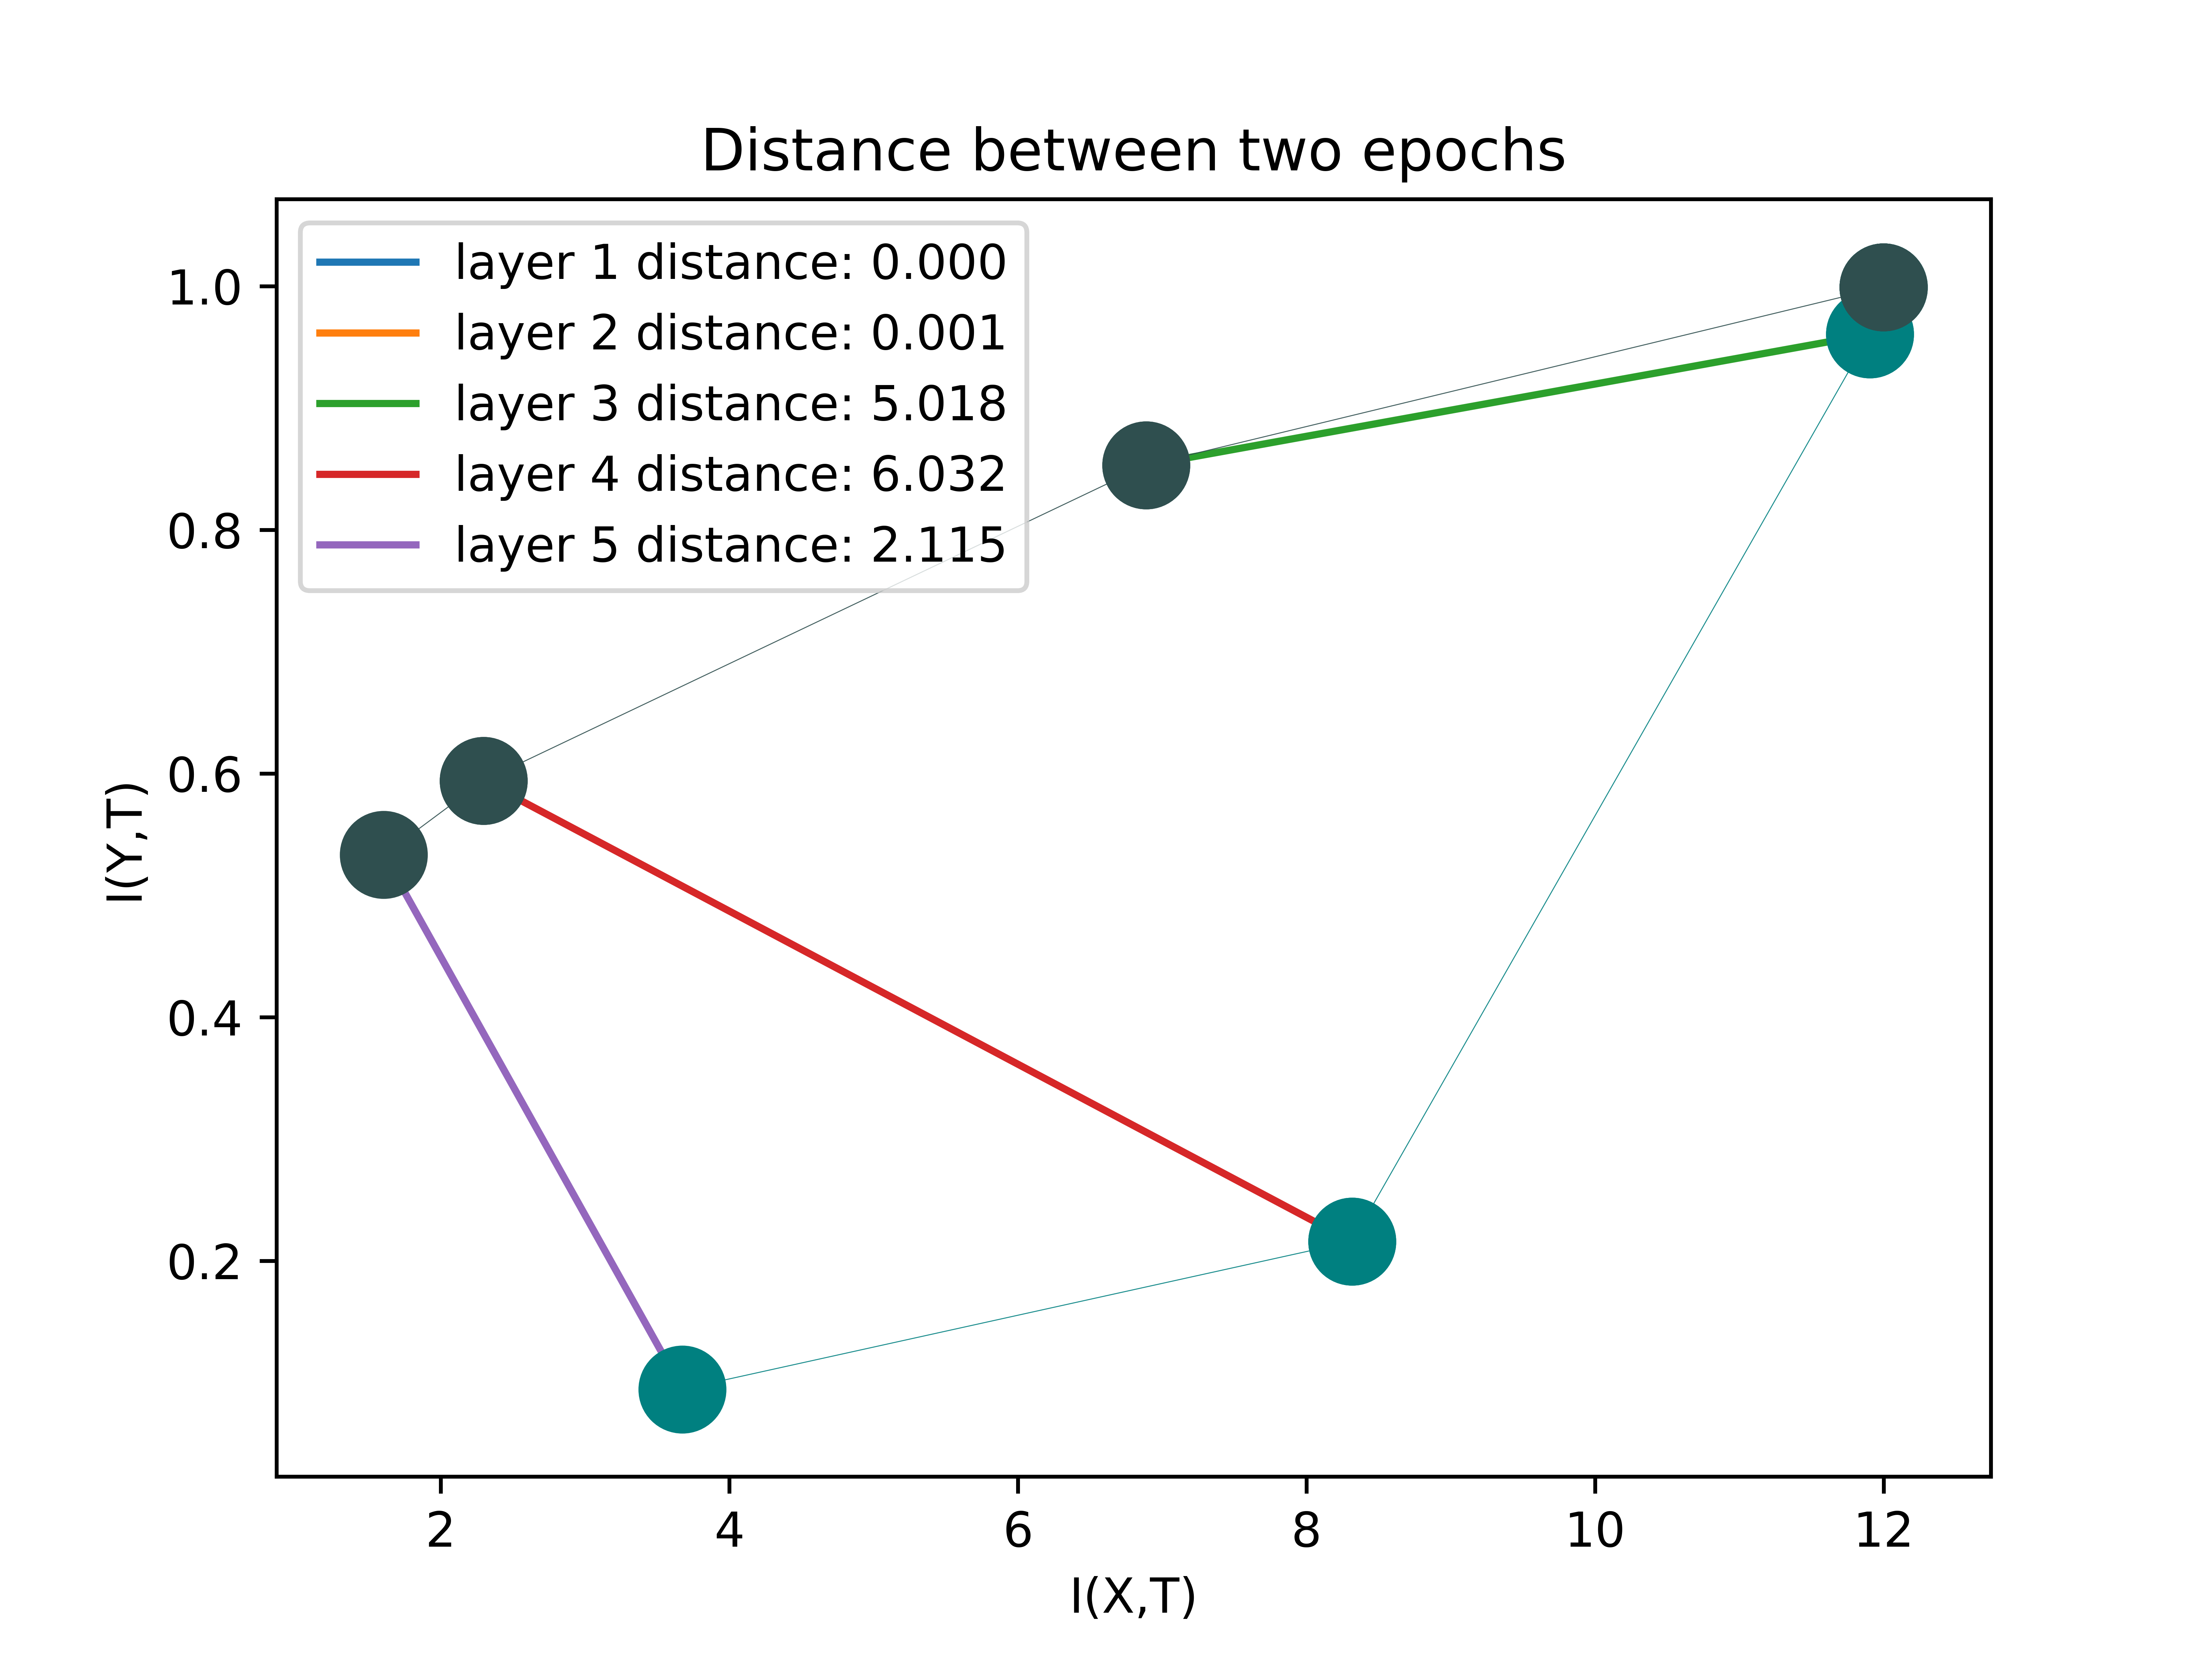
\includegraphics[width=0.80\textwidth]{figs/ip_pair.png}
    \captionof{figure}{
      Example how distance between two epochs is measured.
    }
    \label{fig:ip_pair}
  \end{figure}

\subsubsection{Delta Skip -- Approximate}

  The Exact method suffers the same problem as when we try to instantiate too
  many mutual information calculation instances, namely it runs out of memory if
  our dataset is too big. In order to solve this we use the approximate method
  which follows closely the Exact method. 

  The Algorithm -- refer to \autoref{fig:deltaapprox}, as previously, in the
  Exact method it uses a distance metric and measures every $n'th$ epoch where
  $n$ is adaptive and depends on how close the epochs are. The critical
  difference between Exact and Approximate method happens when the distance
  between epochs is more than $\delta$, the Exact method attempts to backtrack
  and fill in the gap whereas the Approximate doesn't backtrack and just
  continues to the next epoch, this is justified because the approximate method
  assumes that distance between epochs only shrinks and never increases.

  This method does not suffer from memory issues but cannot be parallelized as
  in order to compute next epoch we need to know the distance between current
  epoch and the previous one. Delta Approximate method performs best when paired
  with highly parallel Mutual Information Estimator.

\begin{figure}[H]
    \begin{pythonfigure}
      Algorithm: Delta Skip - Approximate
      Input:
      prev = mutual information result of the previous epoch
      curr = mutual information result of the current epoch
      ;$\delta$; = user specified estimated "distance" between epochs
      Output:
      Algorithm:
      dist = Distance(prev, curr)
      if dist > ;$\delta$;:
        skip = skip
      else:
        skip = skip*2
    \end{pythonfigure}
    \caption{Delta Skip Approximate}
    \label{fig:deltaapprox}
\end{figure}

-----------------------------------------------------------------------------

\section{As-If-Random Experiment}

Tishby's paper relies heavily on the notion that weights of a neural network
behave `as if' they are random, however his and Saxe's experiments don't capture
this idea as much as they could -- refer to \autoref{ssection:rename}. 

An experiment that better captures the ideas of random is instead of 


\begin{itemize}
  \item{
      Tishby and Saxe didn't capture randomness incredibly well 
    }
  \item{
      We have a bettter way
    }
  \item{
      How we've done it, only measure compression at the end of the training
      period when the network is stable and only "brownian randomness
      happens"(refer paper what randomness).
    }
  \item{
      the problem is every x in X is unique, if we sample multiple epochs
      instead of only one we have more compresssion
    }
  \item{
      we rely on the property of the network that there is very little change at
      the end of the training period
    }
  \item{
      Achieves compression even with ReLu yay!!!!!!!!!
    }
\end{itemize}


We believe that Tishby's experiments Saxe's experiments could be improved, with
introducing a better notion of randomness. blah blah blah blah not finished.


\section{Repository Structure}
